\documentclass[english, a4paper]{article}

\usepackage[T1]{fontenc}    % Riktig fontencoding
\usepackage[utf8]{inputenc} % Riktig tegnsett
\usepackage{babel}   % Ordelingsregler, osv
\usepackage{graphicx}       % Inkludere bilder
\usepackage{booktabs}       % Ordentlige tabeller
\usepackage{url}            % Skrive url-er
\usepackage{textcomp}       % Den greske bokstaven micro i text-mode
\usepackage{units}          % Skrive enheter riktig
\usepackage{float}          % Figurer dukker opp der du ber om
\usepackage{lipsum}         % Blindtekst
\usepackage{subcaption} 
\usepackage{amssymb}
\usepackage{color}
\usepackage{amsmath}  
\usepackage{braket} 
\usepackage{multicol}
%\usepackage[]{mcode}

% add source code in box
\usepackage{xcolor}
\usepackage{listings}
\usepackage{caption}
\DeclareCaptionFont{white}{\color{white}}
\DeclareCaptionFormat{listing}{%
  \parbox{\textwidth}{\colorbox{gray}{\parbox{\textwidth}{#1#2#3}}\vskip-4pt}}
\captionsetup[lstlisting]{format=listing,labelfont=white,textfont=white}
\lstset{frame=lrb,xleftmargin=\fboxsep,xrightmargin=-\fboxsep}

\usepackage{amsfonts}
\usepackage{setspace}
\usepackage[cm]{fullpage}		% Smalere marger.
\usepackage{verbatim} % kommentarfelt.
\setlength{\columnseprule}{1pt}	%(width of separationline)
\setlength{\columnsep}{1.0cm}	%(space from separation line)
\newcommand\lr[1]{\left(#1\right)} 
\newcommand\lrb[1]{\left[#1\right]} 
\newcommand\bk[1]{\langle#1\rangle} 
\newcommand\uu[1]{\underline{\underline{#1}}} % Understreker dobbelt.



% JF i margen
\makeatletter
\makeatother
\newcommand{\jf}[1]{\subsubsection*{JF #1}\vspace*{-2\baselineskip}}

% Skru av seksjonsnummerering (-1)
\setcounter{secnumdepth}{3}

\begin{document}
\renewcommand{\figurename}{Figure}
% Forside
\begin{titlepage}
\begin{center}

\textsc{\Large FYS4460}\\[0.5cm]
\textsc{\Large Spring 2016}\\[1.5cm]
\rule{\linewidth}{0.5mm} \\[0.4cm]
{ \huge \bfseries Project 4}\\[0.10cm]
\rule{\linewidth}{0.5mm} \\[1.5cm]

% Av hvem?
\begin{minipage}{0.49\textwidth}
    \begin{center} \large
        John-Anders Stende \\[0.8cm]
    \end{center}
\end{minipage}


\vfill

% Dato nederst
\large{Date: \today}

\end{center}
\end{titlepage}


\textit{Measure} $n(s,p_c,L)$ \textit{and find a finite scaling theory and demonstrate the theory by a finite
scaling data collapse} \\

\section{Cluster number density}
Cluster number density $n(s,p)$ er definert som sannsynligheten for at en site er en spesifikk
site i en cluster av størrelse / masse $s$. $n(s,p)$ er altså cluster size-distribusjonen: Vi kan 
lage et histogram av cluster-størrelser, dvs. hvor mange clusters som er av størrelse $s$ for flere $s$.
$n(s,p)$ kan måles slik:
\begin{equation}
 \overline{n(s,p)} = \frac{N_s}{L^d}
\end{equation}
der overlinen betyr at dette er en målt, ikke eksakt størrelse, $N_s$ er antall clusters av størrelse $s$, 
$L$ er størrelsen til system og $d$ er dimensjonen. Formen til $n(s,p)$ vil være konstant / lineær til vi kommer til
et visst punkt, der den faller raskt. Vi kan dermed definere en cut-off cluster-størrelse, eller en såkalt
karakteristisk cluster-størrelse:
\begin{equation}
 s_\xi \propto |p - p_c|^{-1/\sigma}
\end{equation}
som viser hvordan denne størrelsen divergerer når $p \to p_c$. $\sigma$ er en unviersell eksponent, dvs.
at den ikke avhenger av detaljene til latticen, men den avhenger av dimensjonaliteten. 
Det er en såkalt kritisk eksponent, som beskriver et fysisk system nære en faseovergang. 
I perkolasjonsteori er denne faseovergangen at systemet går fra å ikke perkolere til å perkolere, dvs.
når $p \to p_c$. Systemet kan alltid beskrives ved en potensfunksjon med en kritisk eksponent
rundt en slik faseovergang. Ved slike overganger kan alle perkolasjonsvariablene redefineres vha.
dimensjonsløse størrelser, dvs. ratioer av potenser av disse dimensjonsløse størrelsene. 
Disse kalles skaleringsfunksjoner. 
$n(s,p)$ kan bli uttrykt generelt på følgende måte:
\begin{equation}
 n(s,p) = s^{-\tau}F(s/s_{\xi})
 \label{generalNumberDensity}
\end{equation}
der $\tau = 2$ i to dimensjoner. $F(s/s_{\xi})$ er en skaleringsfunksjon, her er $s$ reskalert som
$s/s_\xi$, og vi er kvitt avhengigheten av $p$, altså vil alle kurvene for forskjellige
$p$ falle på hverandre, dette kalles datakollaps. Det avhenger imidlertid av at de kritiske eksponenten er 
riktige. Dette kan også brukes til å \textit{finne} de kritiske eksponentene ved å plotte $n(s,p)$
helt til alle kurvene faller oppå hverandre. Poenget med skaleringsfunksjonene er at de er uavhengige av
systemstørrelse $L$ og sannsynligheten $p$, men sterkt avhengige av alle andre parametre. Altså vil 
data for forskjjelige $L$ og $p$ kollapse på samme kurve dersom parametrene er valgt riktig. 

\subsection{Måle cluster number density}
$n(s, p_c, L)$ kan måles ved å realiserer et system $M$ ganger, måle $N_s$ for hver realisering og
deretter regne ut
\begin{equation}
 \overline{n(s,p)} = \frac{N_s(M)}{L^2 \cdot M}
\end{equation}
der $N_s(M)$ er antall clusters av størrelse $s$ målt i $M$ realiseringer av perkolasjonssystemet. 
Vi vil altså måle for forskjellige $L$ ved perkolasjonsterskelen $p_c$. Først initaliserer vi
\begin{lstlisting}
M = 100;       % number of realizations / measurements
L = [25 50 100 200 400 800];
pc = 0.59275;      % percolation treshold
allarea = [];      % areas of all clusters sampled M times
\end{lstlisting}
Så looper vi gjennom alle $L$, $M$ ganger:
\begin{lstlisting}
for j = 1:length(L)
    for i = 1:M
        z = rand(L(j),L(j));
        m = z < pc;
\end{lstlisting}
Her lager vi en random matrise av størrelse $L \times L$, og finner så alle occupied sites, dvs.
alle sites som har et tall mindre enn $p_c$. 
Clusterne identifiseres slik:
\begin{lstlisting}
        % lw: each occupied site is given an index that says
        % which cluster it belongs to
        [lw, num] = bwlabel(m,4);
\end{lstlisting}
der 4 betyr nærmeste-nabo-konvensjon. 
Deretter finner vi evt. spanning clusters og 
fjerner dem: HVORFOR GJØR VI DETTE???
\begin{lstlisting}
         % find and remove spanning cluster
        top = lw(1,:);
        bottom = lw(L(j),:);
        left = lw(:,1);
        right = lw(:,L(j));
        tb = intersect(top,bottom);
        lf = intersect(left,right);
        sc = union(tb,lf);
        % remove sites that are not part of clusters
        % sc now contains the indicies of eventual spanning clusters
        sc = sc(sc~=0);
        if ~isempty(sc);
            for k = 1:length(sc);
                % remove spanning clusters
                %length(sc)
                lw = lw(lw ~= sc(k));
            end
        end
\end{lstlisting}
Deretter finner vi antall sites i hver cluster, dvs. $N_s$:
\begin{lstlisting}
         % find distribution of cluster sizes
        s = regionprops(lw, 'Area');
        % area contains number of sites in all clusters
        area = cat(1, s.Area);
        allarea = cat(1, allarea, area);
\end{lstlisting}
For små $s$ har vi god statistikk; mange clusters er på noen få sites. For store $s$ er det imidlertid veldig få,
et histogram vil derfor kun ha et datapunkt i mange bins for store $s$. Vi vil derfor ha større binstørrelse
for større $s$. Dette kan oppnås ved logaritmisk binning, dvs at binkantene er $a^i, \quad i = 0, 1, 2, \dots$.
Da er det viktig å huske på å dele antallet clusters i hver bin med binstørrelse! 
\begin{lstlisting}
    % logarithmic binning
    % n: vector of number of elements in each bin
    % s: location of all bin centers
    [n,s] = hist(allarea, L(j)^2);
    a = 1.2;                                % basis for logartithmic bins
    logamax = ceil(log(max(s)) / log(a));   % edge of largest bin
    bins = a.^(0:1:logamax);                % bin edges
    nl = histc(allarea, bins);              % histogram with new bins
    ds = diff(bins);                        % bin sizes
    sl = (bins(1:end-1) + bins(2:end))*0.5; % bin centers
    nsl = nl(1:end-1)'./(M*L(j)^2*ds);         % cluster number density
    legendInfo{j} = sprintf('p = %.2f', p(j));
    loglog(sl, nsl);
    hold on;
\end{lstlisting}
For alle $L$ gjør vi et loglog-plot. Når vi ikke gjør datakollaps ser det slik ut:
\begin{figure}[H]
  \begin{center}
  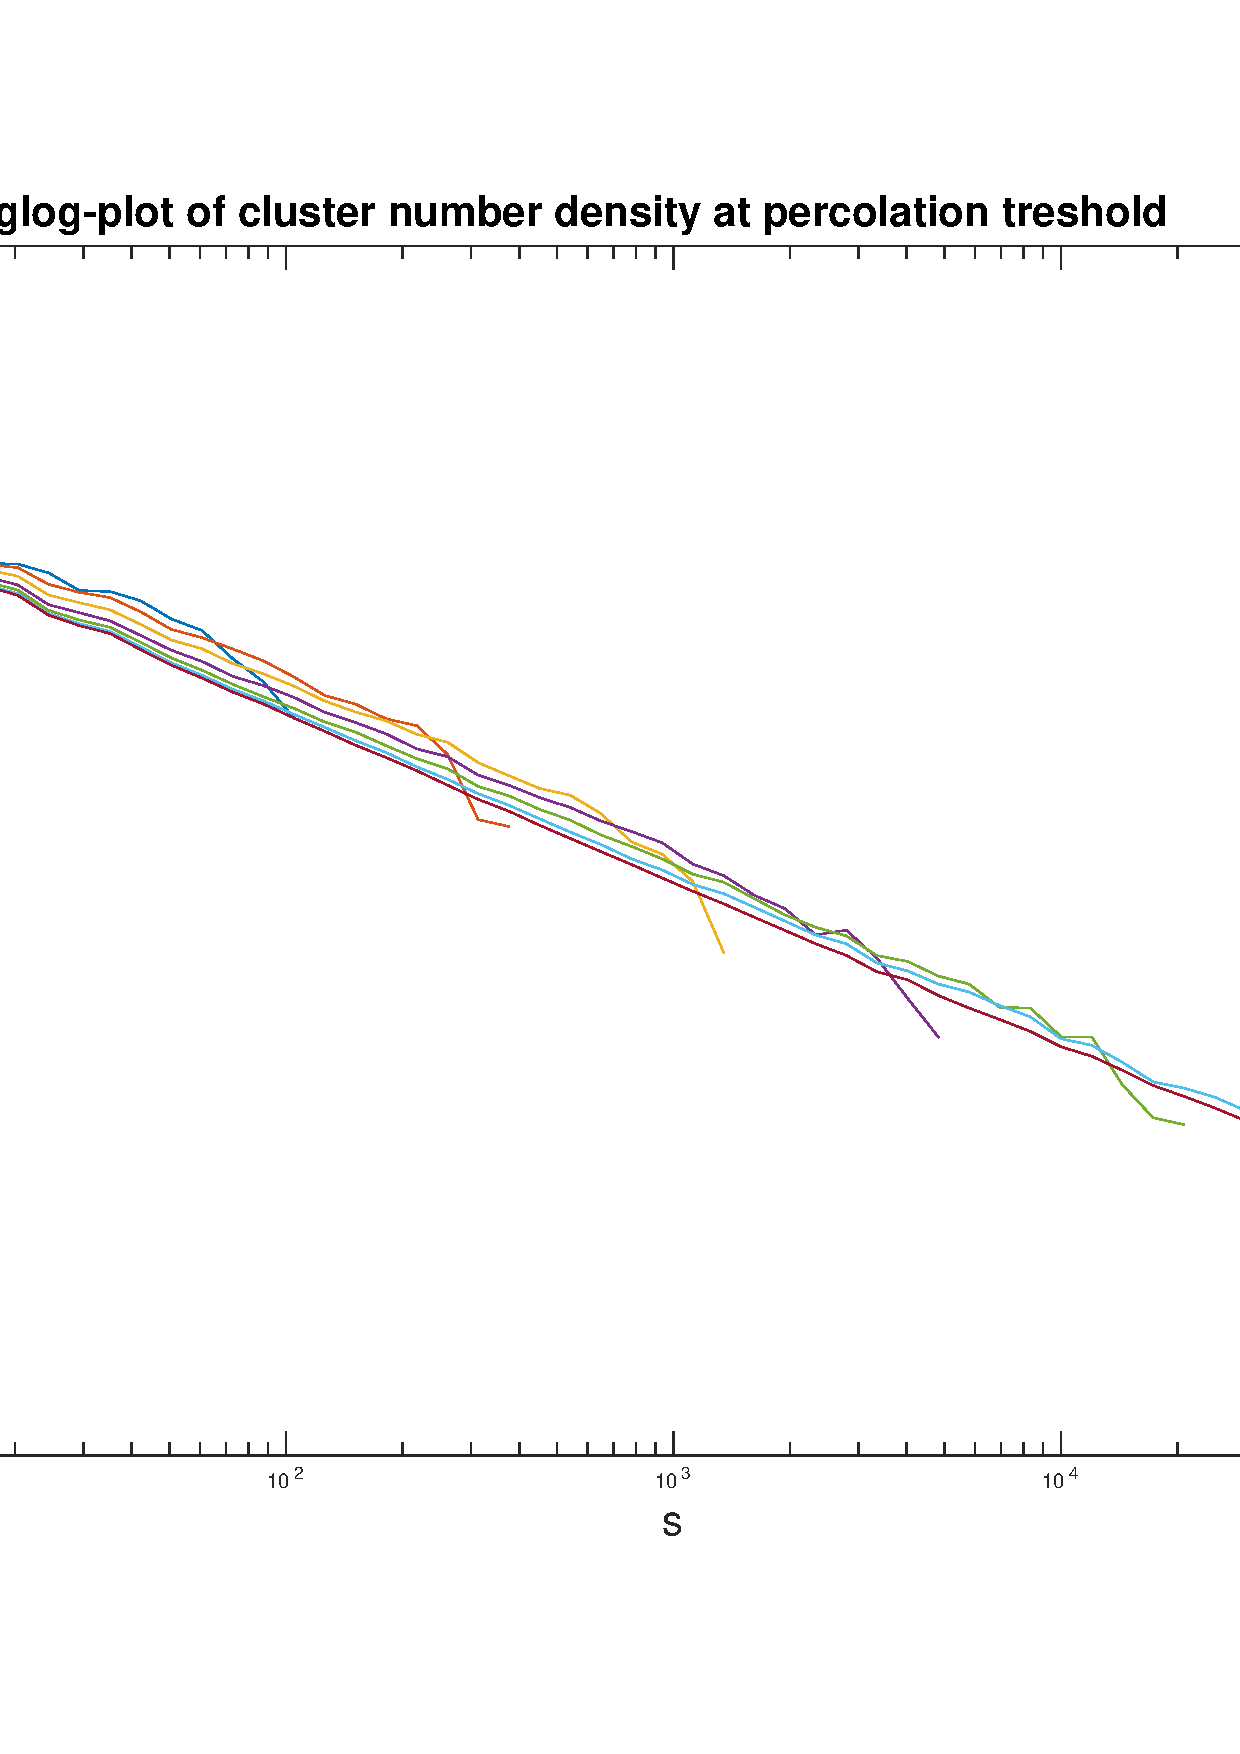
\includegraphics[width = 140mm]{../Figures/clusterNumberDensity3.png}
  \caption{Cluster number density for $p_c$ som funksjon av $L$.}
  \label{fig:fig1}
  \end{center}
\end{figure}
Vi ser at formen til $n(s,p_c,L)$ nettopp er som i \eqref{generalNumberDensity} : 
For lave $s$ går funksjonen som $s^{-\tau}$, før den faller eksponentielt
ved det kritiske punktet. Her er det skaleringsfunksjonen $F$ som bestemmer oppførselen. 

\section{Finite size skalering}
Vi må utvikle en finite size-skaleringsteori for å finne skaleringsfunksjonen. 
Her tar vi hensyn til at systemet er av endelig størrelse, dvs. $L$ er ikke uendelig stor. 
Vi har altså at 
\begin{equation}
 n(s,p) = s^{-\tau}F(s/s_\xi)
\end{equation}
Vi vet også at det det er kun er én eneste karakterisk størrelse av en cluster:
\begin{equation}
 s_\xi \propto \xi^D
\end{equation}
der $\xi$ er korrelasjonslengden, dvs. cut-off til korrelasjonsfunksjonen $g(r)$ som sier
hva sannsynligheten for at to okkuperte sites i avstand $r$ er i samme cluster. 
Dermed har vi
\begin{equation}
 n(s,p) = s^{-\tau}F(s/\xi^D)
\end{equation}
Vi har to ulike paradigmer når for endelige systemstørrelser $L$:
\begin{equation}
 s^\tau n(s,p) = 
 \begin{cases}
 F(s/L^D) & L \ll \xi \\
 F(s/\xi^D) & L \gg \xi
 \end{cases}
\end{equation}
dvs. når $L \ll \xi$ vil vi typisk se en spanning cluster, fordi den typiske størrelsen av en cluster
er større en systemstørrelsen. Vi kan imidlertid ikke vite om vi er ved $p=p_c$ eller ikke, bare
at $p_c$ er et eller anet sted for $\xi(p) > L$. I dette tilfellet vil derfor den typiske cluster-størrelsen
være lik systemstørrelsen:
\begin{equation}
 \xi \propto L
\end{equation}
Vi skal måle $n(s, p_c, L)$, vi er altså på $p=p_c$. Vi vet at $\xi$ divergere som en potensfunksjon
når $p \to p_c$:
\begin{equation}
 \xi \propto |p-p_c|^{-\nu}
\end{equation}
derfor har vi $\xi = \infty$ nå. Altså er vi i området $L \ll \xi$, derfor er skaleringsfunksjonen til 
$n(s,p)$ gitt som
\begin{equation}
 s^{\tau} n(s,p, L) = F(s/L^D)
\end{equation}
Det betyr at dersom vi måler $n(s,p_c,L)$ som ovenfor og plotter $\textrm{log}_{10}[s^\tau n(s,p_c,L)]$ mot
$\textrm{log}_{10}[sL^{-D}]$, vil vi få en datakollaps. Dette vil demonstrere finite size-skaleringsteorien.
Vi brukte de gitte verdiene $\tau = 187/91$ og $D = 91/48$ (disse kan også måles ved simuleringer).
\begin{figure}[H]
  \begin{center}
  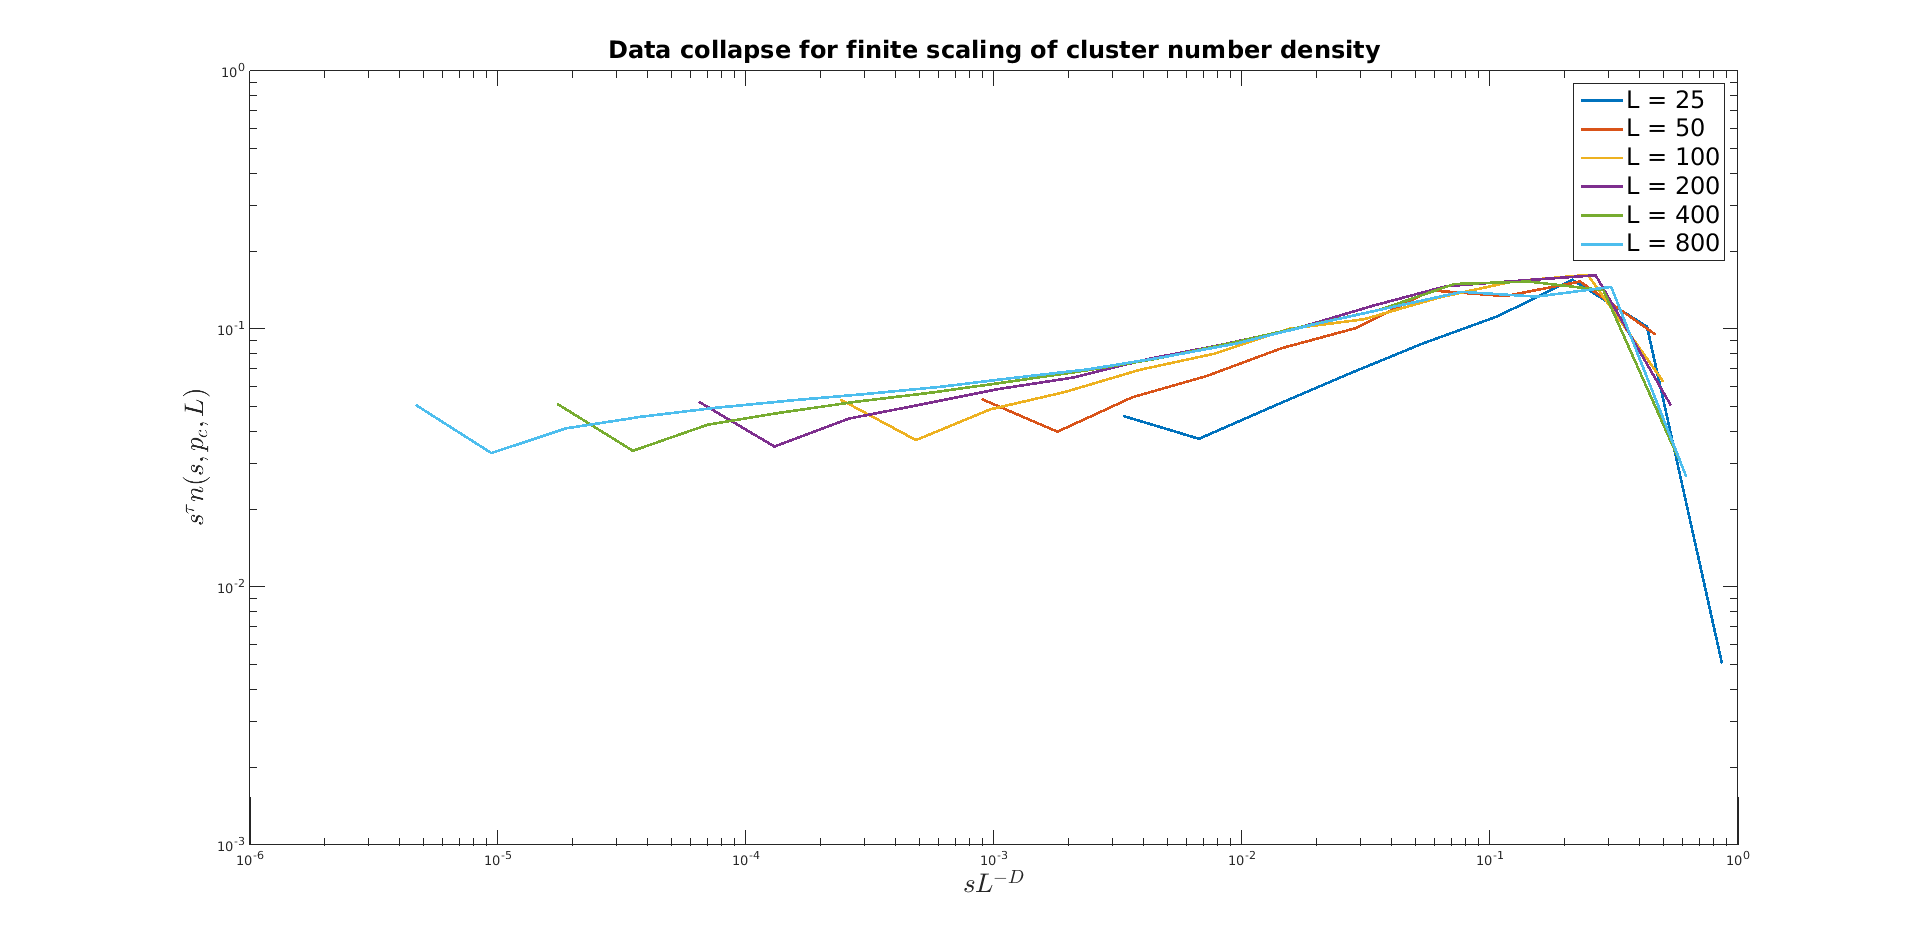
\includegraphics[width = 140mm]{ndcDataCollapse.png}
  \caption{Cluster number density for $p_c$ som funksjon av $L$.}
  \label{fig:fig1}
  \end{center}
\end{figure}
Hvis man bruker andre verdier for de kritiske eksponentene enn de ovenfor, ser vi at det ikke blir datakollaps:
\begin{figure}[H]
\begin{minipage}[t]{0.48\linewidth}
  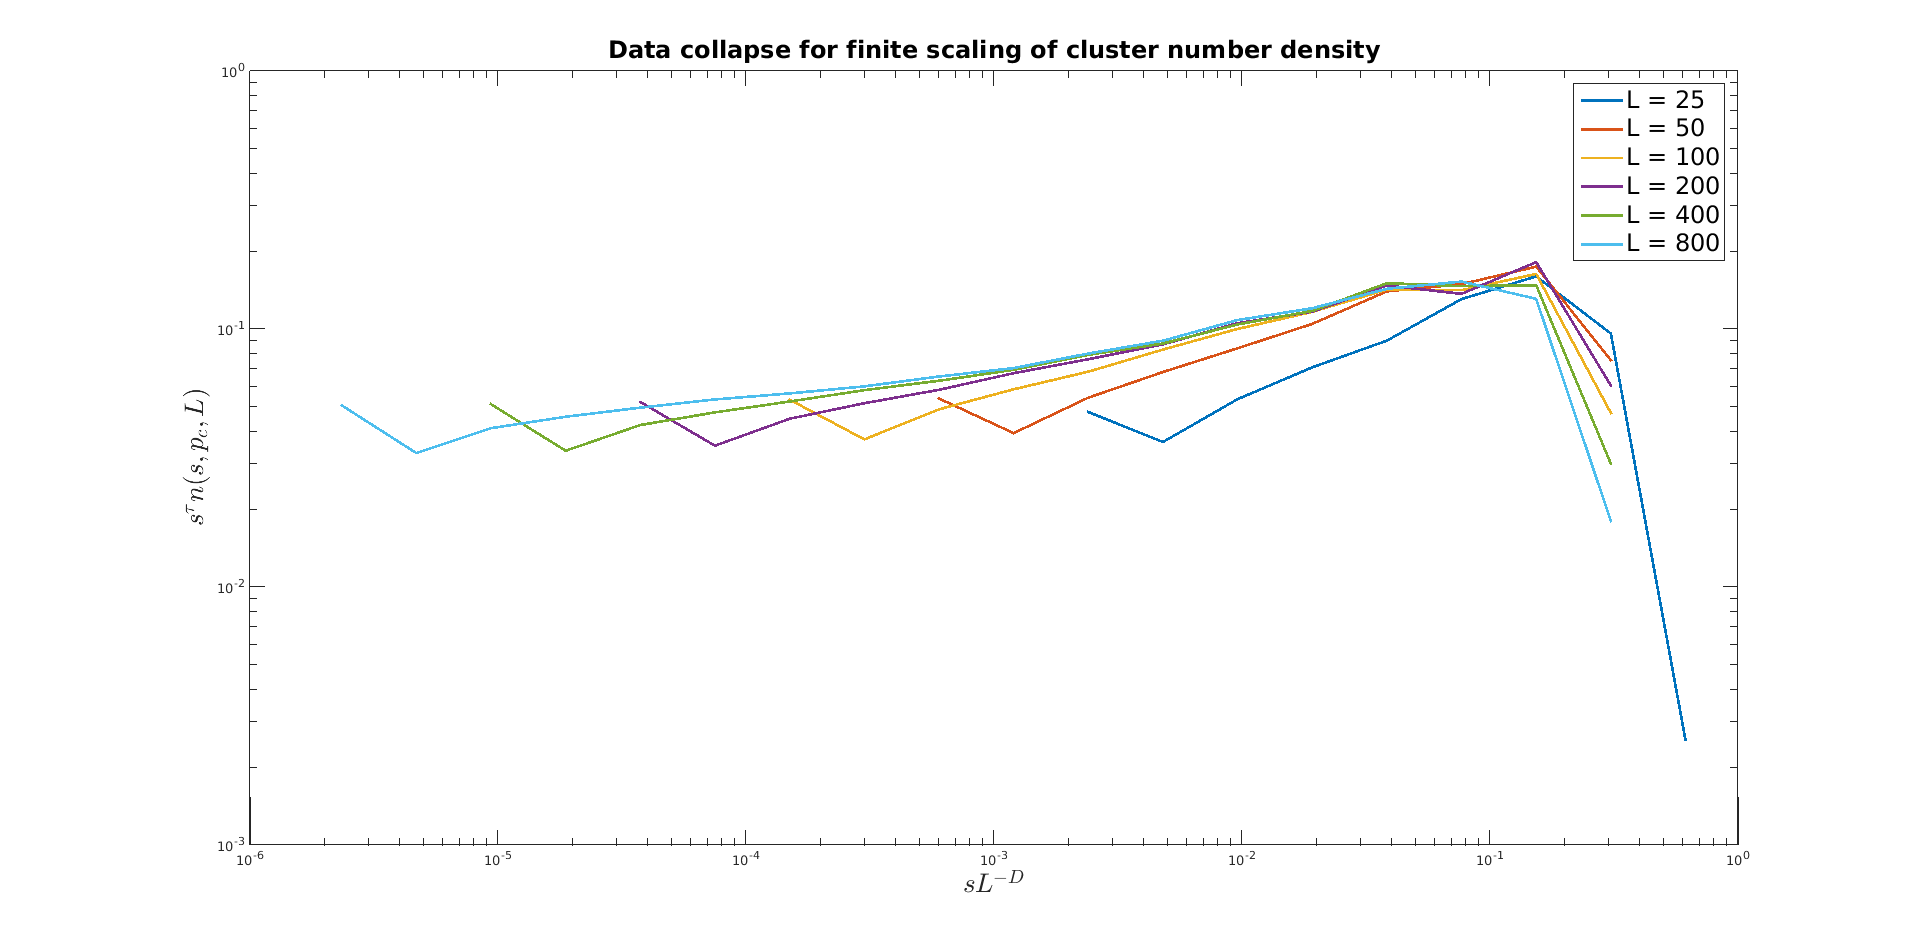
\includegraphics[width=\textwidth]{cndDataCollapseD2.png}
  \caption{$D=2.0$, $\tau = 187/91$}
  \label{fig:minipage1}
\end{minipage}
\quad
\begin{minipage}[t]{0.48\linewidth}
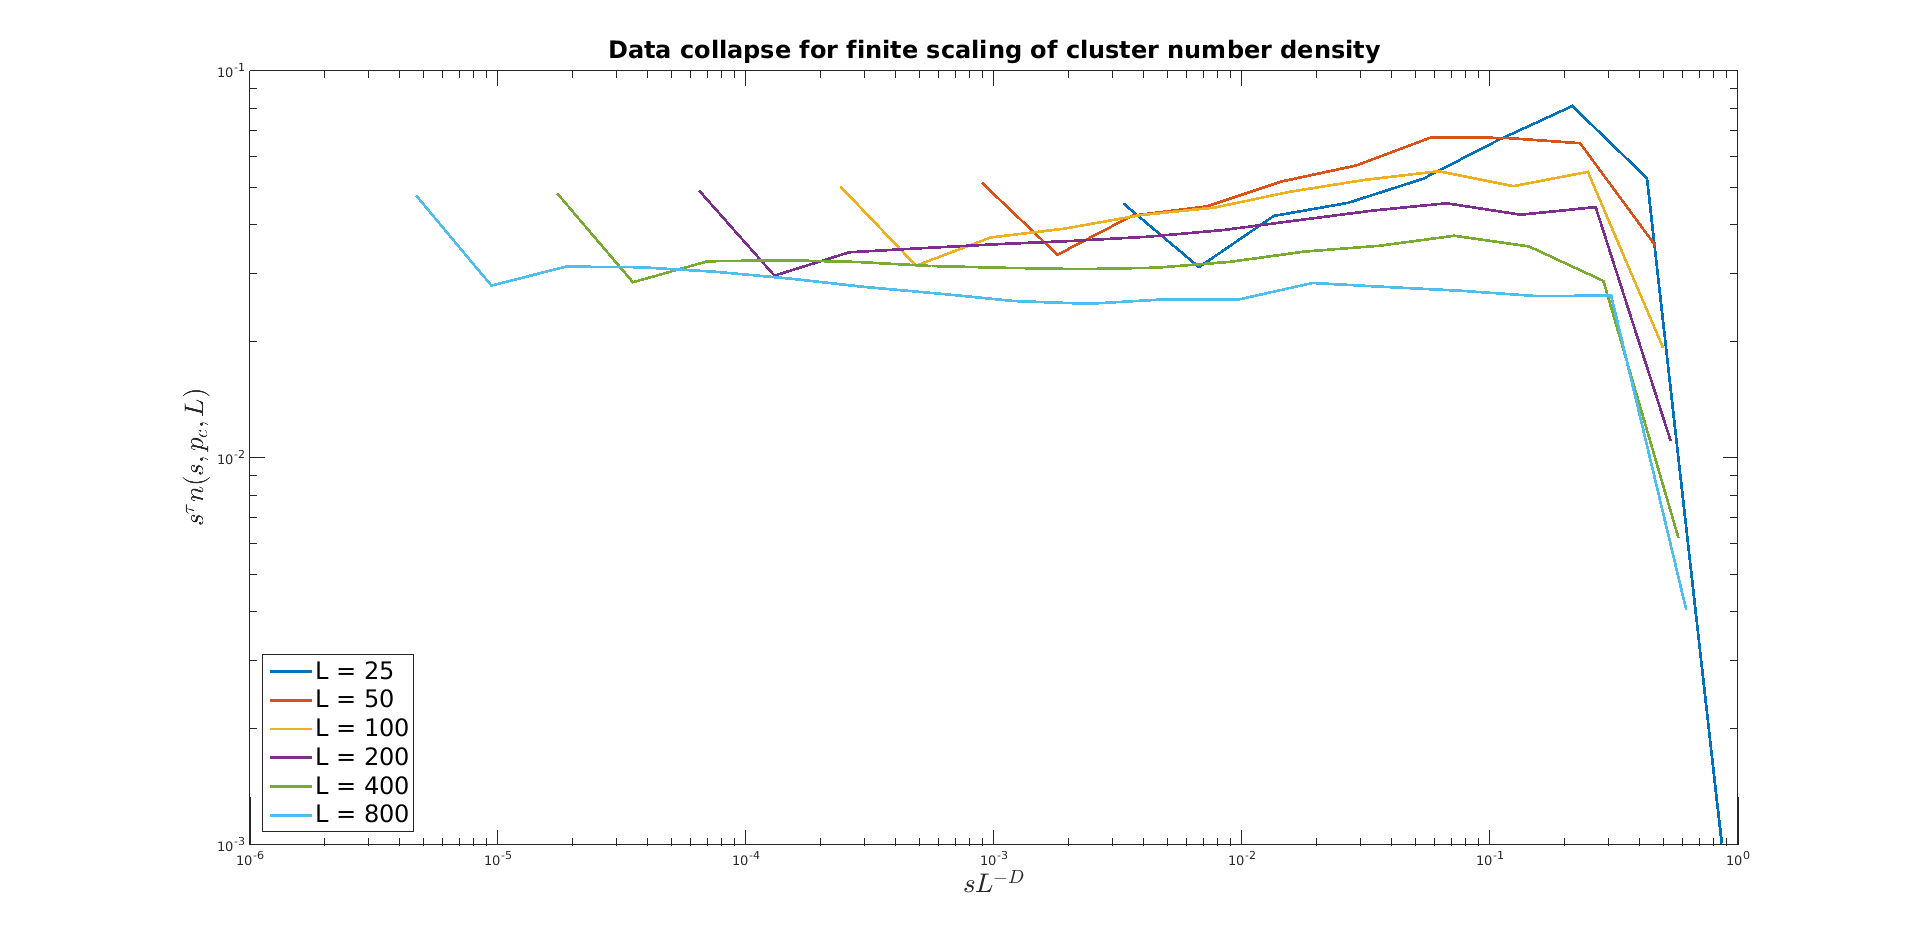
\includegraphics[width=\textwidth]{cndDataCollapseTau19.png}
  \caption{$D=91/48$, $\tau = 1.9$}
  \label{fig:minipage1}
\end{minipage}
\end{figure}

\begin{figure}[H]
  \begin{center}
  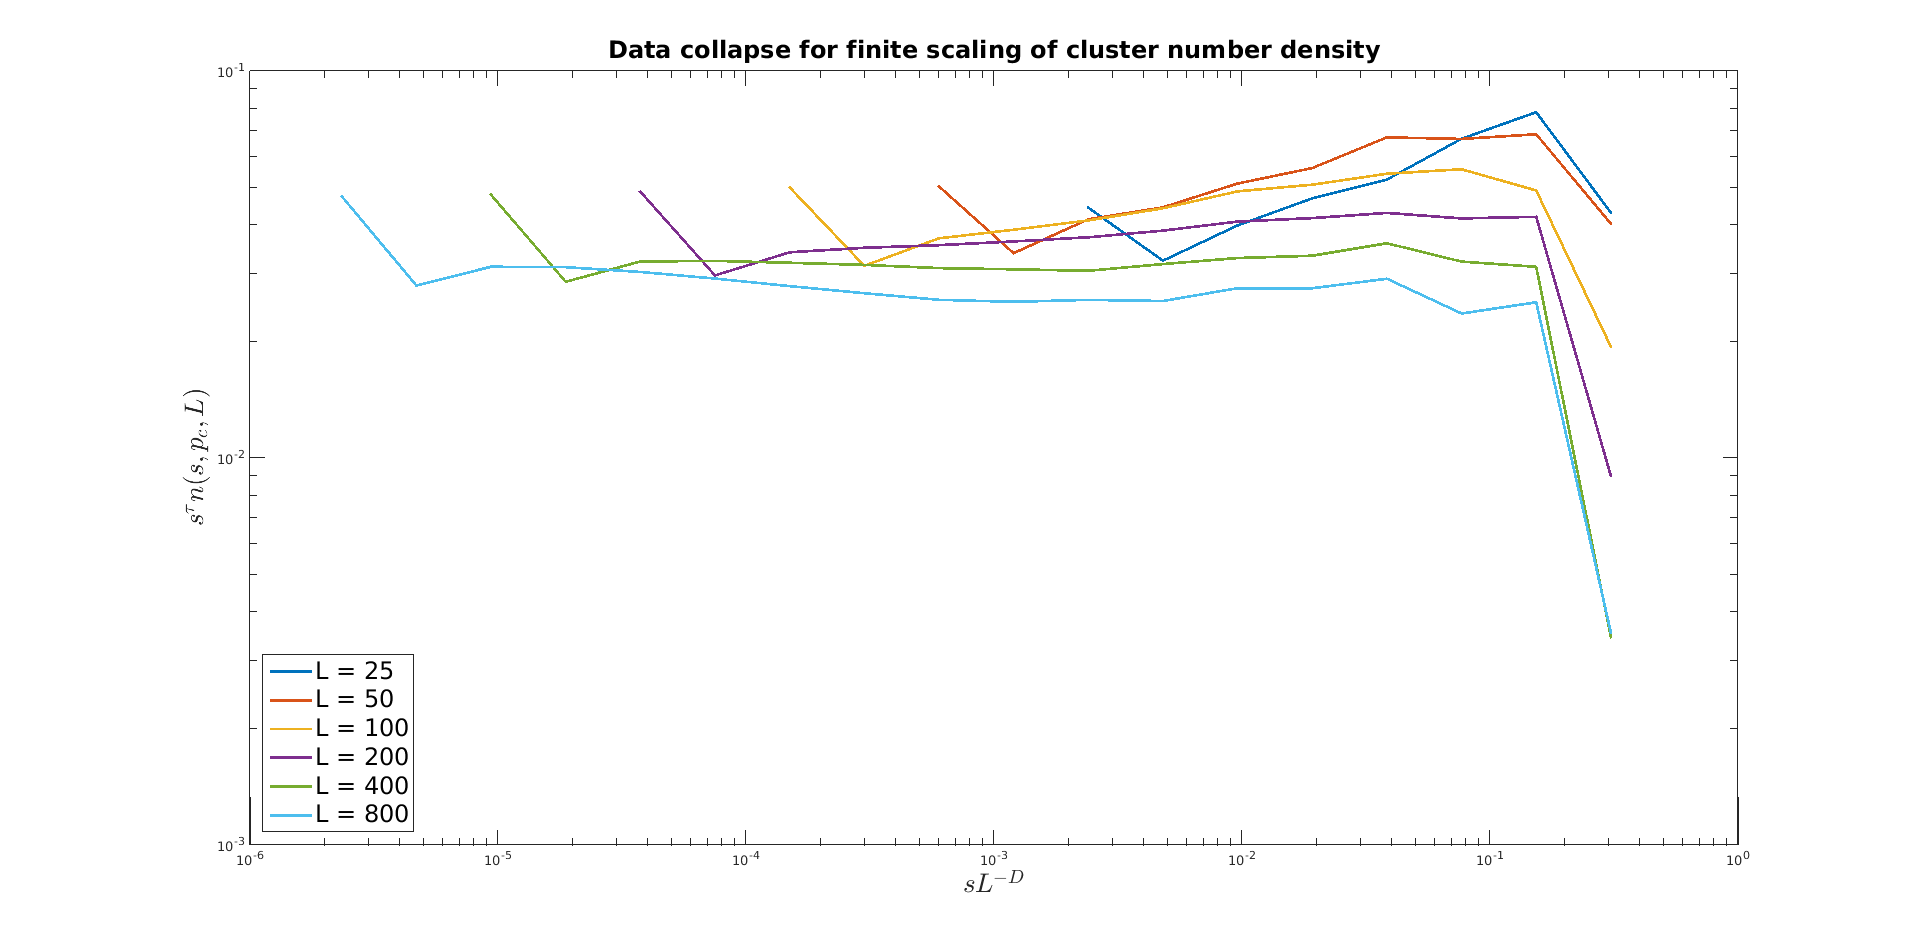
\includegraphics[width = 140mm]{cndDataCollapseD2Tau19.png}
  \caption{$D=2.0$, $\tau = 1.9$}
  \label{fig:fig3}
  \end{center}
\end{figure}


JEG MÅ SI NOE OM HVORDAN DETTE ENDRER SEG MED DIMENSJONER. D AVHENGER VEL AV DIMENSJONEN?







\end{document}
